\clearpage
\section{Soft- und Firmware}\label{sec:Soft-undFirmware}


Im folgenden Abschnitt werden Anforderungen, Konzept, Entscheidung und die Umsetzung der Software dokumentiert. Die Lösungsfindung und ihre Prozess wird nachfolgend beschrieben. 

\subsection{Anforderungen}\label{subsec:Software_Anforderungen}

Wie bereits im Abschnitt \ref{sec:Abgrenzung} wurden die Anforderungen in der Aufgabenstellung (siehe Anhang \ref{app:Aufgabenstellung}) sowie im Pflichtenheft (siehe Anhang \ref{app:Pflichtenheft}) vorgängig festgelegt. Im Fokus steht das erfassen der wichtigsten Messgrössen welche nachfolgend aufgeführt werden. \\

\begin{itemize}
	\item \textbf{Latenzzeit}: Bestimmung der Latenzzeit in Millisekunden zwischen den Teilnehmern. Die Genauigkeit sollte bei $+/-$1 ms liegen.  
	\item \textbf{Anzahl Hops}: Bestimmung der Anzahl Hops, über welche eine Nachricht übermittelt wird.
	\item \textbf{Datenrate}: Messen der Datenrate in Bytes/s, welche zwischen zwei Teilnehmern erreicht wurde. 
	\item \textbf{RSSI}: Erfassen des RSSI-Werts der eingehenden Pakete.
	\item \textbf{Paketverlust}: Pakete zählen, welche ihr Ziel nicht erreicht haben.  
	\item \textbf{Aktive Radio Zeit}: Erfassen der aktiven Radio-Zeit um den Energieverbrauch abschätzen zu können. 
\end{itemize}


Die Erfassung muss in allen Mesh-Netzwerken möglich sein. Um die Messresultate vergleichen zu können müssen die gleichen Ausgangslagen vorliegen, sowie die selben Messmethoden angewendet werden. 

\todo[inline]{Beschreiben der Anforderungen an die Software. Einzelne Teilprobleme Beschreiben}


\subsection{Konzept}\label{subsec:Software_Konzept}

Um die Messdaten erfassen zu können müssen alle Teilnehmer im Netzwerk eine eigenes Log führen. Dieses wird im Anschluss an eine zentrale Auswerte-Stelle übermittelt um ausgewertet zu werden (wie in Abschnitt ... beschrieben). Folgende Daten müssen pro eingehende oder gesendete Nachricht von allen Teilnehmern der Messung erfasst werden. 

\begin{itemize}
	\item \textbf{Message-ID}: Eindeutige Kennung (Laufnummer) welche beim Senden einer Nachricht mitgegeben wird. Somit können die Nachrichten anschliessend zugeordnet werden. 
	\item \textbf{Timestamp}: Erfassen der Sende- / Empfangszeit über synchronisierten Zeitwert. Relevant zur Bestimmung der Latenzzeit und Datenrate. 
	\item \textbf{Hops}: Auslesen der Anzahl Hops des Pakets beim Empfangen. Beim Senden kann dieser Wert ignoriert werden.
	\item \textbf{Source Address}: Erfassen der Teilnehmer-Addresse welcher die Nachricht sendet oder gesendet hat. Wichtig für die korrekte Zuordnung der Pakete. 
	\item \textbf{Destination Address}: Erfassen der Teilnehmer-Addresse welcher die Nachricht empfangen hat. Ebenfalls für Zuordnung der Nachrichten relevant. 
	\item \textbf{Group Address}: Erfassen der Gruppen-Adresse in welcher die Nachricht unterwegs war. Notwendig zur Erfassung des Paketverlustes. 
	\item \textbf{RSSI}: Erfassen des RSSI-Werts der eingehenden Pakete. Beim senden soll dieser Wert 0 sein. 
	\item \textbf{Paketgrösse}: Erfassen der Paketgrösse um die Datenrate zu berechnen. 
\end{itemize}

Zur Steuerung der Messungen wird eine zentrale Stelle (Master) verwendet (Wie in Abschnitt ... beschrieben). Diese soll einzelne Teilnehmer Konfigurieren, eine Messung starten, sowie die Reports  einsammeln können. 


\todo[inline]{Konzept zur Lösung der Teilprobleme grob beschreiben}


\subsection{Entscheidung}\label{subsec:Software_Entscheidung}

Zur Umsetzung der Mesh-Stacks mittles der \textit{NRF-Platform} sind folgende SDKs vorhanden: 

\begin{itemize}
	\item \textit{\textbf{nRF Connect SDK}}: Auf dem Zephyr-RTOS aufbauende SDK. Diese soll in Zukunft alle drei Mesh-Protokolle (Bluetooth-Mesh, Openthread und Zigbee) unterstützen. Wird jedoch noch nicht zum Einsatz in End-Produkten empfohlen. \cite{nordic_semi_welcome_to_the_nrf_connect_sdk_2020}
	\item \textit{\textbf{nRF SDK for Thread and Zigbee}}: Proprietäre SDK Library von Nordic Semiconductor. Thread integration mittels Openthread, Zigbee einbindung mittels ZBOSS. \cite{nordic_semi_nrf_sdk_for_thread_and_zigbee_2020}
	\item \textit{\textbf{nRF SDK for Mesh}}: Proprietäre SDK Library von Nordic Semiconductor für Bluetooth-Mesh. Ist zur Produktion freigegeben. \cite{nordic_semi_nrf_sdk_for_mesh_2020}
\end{itemize}

Die Messungen sollten trotz der verschiedenen Bibliotheken möglichst einheitlich sein, um die Vergleichbarkeit nicht zu beeinträchtigen. Daher musste ... Das Erfassen der Daten erfolgt Um eine möglichst unabhängig von der verwendeten Library zu sein wurde auf eine selbst entwickelte Kommunikation über die P2P-Testinfrastruktur gesetzt. 

\todo[inline]{Warum wurde die Software so umgesetzt?}

\todo[inline]{Tabelle der SDKs und Stacks und ihren Möglichkeiten aufzeigen. -> Gesamtheitliche Lösung mittels eigener Verwaltungsschicht und P2P}


\todo[inline]{Tabelle welche Software zu welchem Stack, Referenzen zu Parts}


\subsection{Umsetzung}\label{subsec:Software_Umsetzung}

\todo[inline]{Cyrill Tabelle und subsections, Raffel und Robin Text}



Die Software und Firmware für die Mesh Benchmarks sowie für die P2P Testinfrastruktur setzt sich aus diversen Modulen zusammen. Die Tabelle \ref{tab:UebersichtSoftware} zeigt eine Übersicht der wichtigsten Module und deren Verwendung in den 4 Benchmark Teilen: BLE Mesh, Zigbee, Thread sowie P2P.
Gemeinsame Module auf Firmware Ebene für die BT Mesh und Zigbee Firmware sind im Ordner SharedLib im Github Repository\footnotemark\ zusammengefasst. Aus diversen Gründen wurde die Thread Firmware zu einem grossen Teil in separaten Modulen realisiert. Die nicht Stack spezifischen Teile der Thread Lösung werden als Thread Common zusammengefasst.
Jene Python Scripts für das Benchmark Management stehen im gleichnamigen Ordner auf dem Github Repository zur Verfügung.
Die Stack bezogenen Implementationen der Benchmark Firmware werden in den individuellen Teilen \ref{part:BluetoothMesh}, \ref{part:Thread} und \ref{part:Zigbee} behandelt.


\newcommand{\rotcells}[1]{%
  \rotatebox[origin=c]{90}{ #1 }%
}
\begin{table}[h]
\centering
\begin{tabular}{|c|l|l|c|c|c|c|} 
\cline{4-7}
\multicolumn{1}{l}{} & \multicolumn{2}{l|}{} & \multicolumn{1}{l|}{BT Mesh} & Zigbee & Thread & P2P \\ 
\hline
\multirow{8}{*}{\rotcells{SharedLib}} & Statemachine & bm\_statemachine.c [\ref{subsubsec:Statemachine}]& x & x &  &  \\ 
\cline{2-7}
 & Timesync & bm\_timesync.c [\ref{subsubsec:Timesync}] & x & x &  & x \\ 
\cline{2-7}
 & Control & bm\_control.c [\ref{subsubsec:Control}] & x & x &  & x \\ 
\cline{2-7}
 & Report & bm\_report.c [\ref{subsubsec:Report}] & x & x &  & x \\ 
\cline{2-7}
 & Logging & bm\_log.c [\ref{subsubsec:Logging}]& x & x &  & x \\ 
\cline{2-7}
 & Flash Save & bm\_flash\_save.c [\ref{subsubsec:FlashSave}]& x & x &  &  \\ 
\cline{2-7}
 & CLI & bm\_cli.c [\ref{subsubsec:CLI}]& x & x &  & x \\ 
\cline{2-7}
 & Low Layer Radio & bm\_radio.c [\ref{subsubsec:LowLevelRadio}]& x & x &  &  \\ 
\hline
\multirow{4}{*}{\rotcells{\begin{tabular}[c]{@{}c@{}}Benchmark\\Management \end{tabular}}} & Flash & Flasher.py [\ref{subsubsec:Flash}]& x & x & x &  \\ 
\cline{2-7}
 & Configurator & Configurator.py [\ref{subsubsec:Configurator}]& x & x &  &  \\ 
\cline{2-7}
 & Benchmark & \begin{tabular}[c]{@{}l@{}}Benchmark\_and\_\\Reporter.py [\ref{subsubsec:Report}] \end{tabular} & x & x &  &  \\ 
\cline{2-7}
 & Analysis & Analysis.py [\ref{subsubsec:Analysis}]& x & x & x &  \\
\hline
\end{tabular}
\caption{Übersicht Shared Lib und Benchmark Management Module}
\label{tab:UebersichtSoftware}
\end{table}

Sämtliche Firm- und Software Komponenten die für Mesh Benchmark sowie die P2P Testinfrastruktur nötig sind, können auf dem Github Repository zum Projekt unter folgendem \href{https://github.com/Rouben94/P6_Software}{Link\footnotemark[\value{footnote}]}  eingesehen werden.

\footnotetext{\url{https://github.com/Rouben94/P6_Software} \cite{anklin_bobst_horath_rouben94p6_software_nodate}}




\subsection{Shared Library}\label{subsec:SharedLibrary}

Die \textit{Shared Library} ist die geteilte Bibliothek zwischen allen Mesh-Stacks. Sie beherbergt alle relevanten Module um eine Messung zu Verwalten. Der jeweilige Mesh-Stack ist lediglich für das senden und empfangen von Nachrichten, sowie zum Erfassen der Messdaten zuständig. 


\begin{figure}[H]
	\centering
	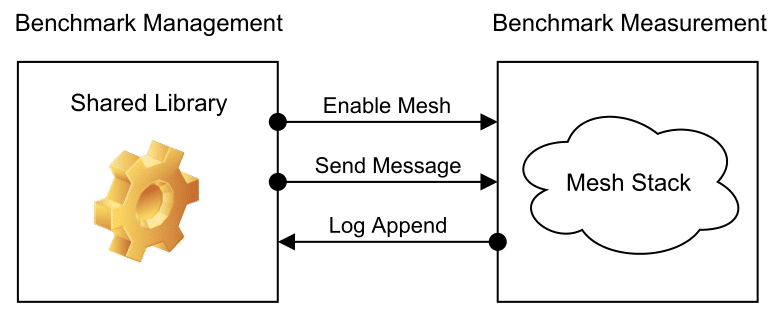
\includegraphics[width=0.6\textwidth]{Shared_Lib_Concept.png}
	\caption{Vereinfachte Anbindung der \textit{Shared Library} an die Mesh-Stacks}\label{fig:ShardeLibConcept}
\end{figure}

Abbildung \ref{fig:ShardeLibConcept} zeigt die vereinfachten Schnittstellen zwischen der Shared-Library und den Mesh-Stacks. Die Bibliothek ist spezifisch für die nRF52840 SOCs zugeschnitten. Um einfach in die jeweilige SDK integrierbar zu sein müssen die Module der Shared-Lib möglichst ohne weitere Abhängigkeiten klar kommen. Sofern Treiber oder externe Bibliotheken für Module benötigt werden, müssen diese von allen SDKs vergleichbar zur Verfügung gestellt werden. Im folgenden Abschnitt wird auf die einzelnen Module der \textit{Shared-Lib} eingegangen. 


\subsubsection{Statemachine}\label{subsubsec:StatemachineSoftware}

Die Statemachine dient dazu den Ablauf, welcher in Abschnitt \ref{subsec:AblaufMesh} beschrieben wurde abzuarbeiten. Sowohl der Master, die Server und Clients arbeiten den in Abbildung \ref{fig:StatemachineFLowgraph} dargestellten Ablauf ab. 

\begin{figure}[H]
	\centering
	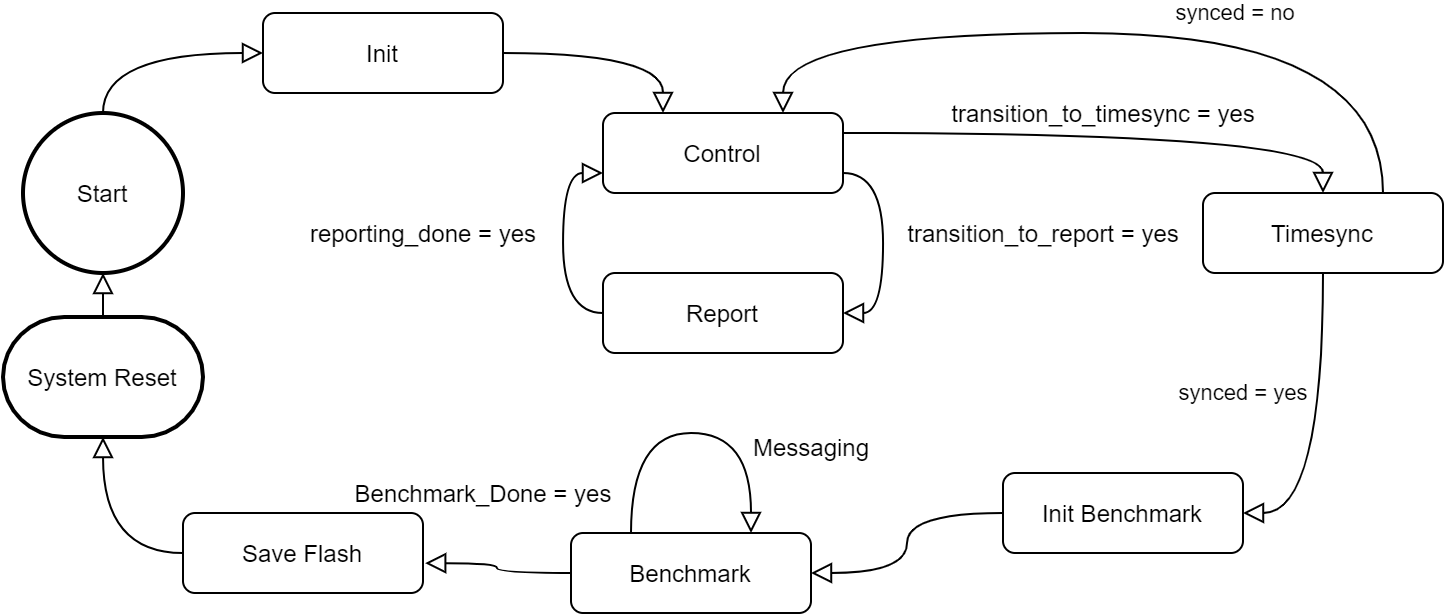
\includegraphics[width=1.0\textwidth]{Statemachine_Flowgraph.png}
	\caption{Flowgraph der Statemachine}\label{fig:StatemachineFLowgraph}
\end{figure}


Die Funktion der Schritte wird im Folgenden grob beschrieben. Zur genauen Untersuchung ist der Source Code unter \cite{rouben94_sharedlib_software_git_2020} verfügbar.  \\

\begin{itemize}
	\item \textbf{\textit{Init:}} Dieser Schritt initialisiert alle notwendige Funktionen (Radio, Timers, usw.). Ebenfalls rekonstruiert dieser Schritt die \textit{Log-Daten} indem er diese aus dem Flash in das RAM kopiert. Nach der erfolgreichen Initialisierung wechselt die Statemachine in den Control-State.
	\item \textbf{\textit{Control:}} Im Control-State wartet jeder Teilnehmer auf eingehende Befehle des Benutzers. Der Master erhält über das Command Line Interface den auszuführenden Befehl. Diesen Befehl wandelt der Master in eine Befehls-Nachricht (Control-Message) um und leitet sie über das Radio-Interface an die Slaves weiter.  Alle Slaves (Clients und Servers) erwarten eine Control-Message über das Radio-Interface. Diese wiederholen die Nachricht, damit sie von weiteren Clients und Servers aufgenommen werden kann.    
	
	
	Der Master verteilt die Zeitsynchronisation an die Slaves. Die Slaves synchronisieren sich auf das Signal des Masters auf, sofern sie in seiner Reichweite liegen. Hat ein Slave sich nicht Synchronisieren können verweilt dieser im \textit{Discovery-State}. Der Master darf immer zum nächsten Schritt voranschreiten. 
	\item \textbf{\textit{Mockup:}} Der Master wartet auf eine Antwort der einzelnen Slaves. Jeder Slave generiert einen zufälligen Timeslot um sich beim Master anzumelden. Der Master führt alle Slaves, welche sich gemeldet haben in einer Liste auf. Ist diese Liste leer (hat sich kein Slave gemeldet), so wird der Master zum \textit{Discovery State} zurückkehren. Ist ein Slave bereits beim Master angemeldet, so muss sich dieser nicht erneut anmelden. 
	\item \textbf{\textit{Param:}} Der Master versendet die Packets-Parameter (Mode, StartChannel, StopChannel, etc) auf welchen er die Probe-Packets versendet. Erhält ein Slave keine Daten so kehrt er in den \textit{Discovery-State} zurück. 
	\item \textbf{\textit{Packets:}} Der Master versendet \textit{Probe Packets} auf den zuvor Kommunizierten Einstellungen. Die Slaves empfangen diese Daten und zählen die Anzahl erfolgreich empfangener Pakete und erfassen weitere Messdaten. 
	\item  \textbf{\textit{Reports Req:}} Nach dem ausmessen beginnt der Master mit dem einsammeln der einzelnen Slave Reports. Dazu sendet er an jeden Slave in seiner Liste (aus dem \textit{Mockup-State}) Report-Anfragen, sogenannte \textit{Reports-Requests}. Die Slaves warten auf einen \textit{Report Request} vom Master. 
	\item  \textbf{\textit{Reports:}} Der Slave, welcher den Request bekommen hat, sendet seinen Report zum Master. Dies muss innerhalb einer gewissen Zeit erfolgen. Sendet ein Slave nach einer gewissen Anzahl von Versuchen keine Reports, wo wird er aus der Liste der gemeldeten Slaves entfernt. Sobald der Master alle Reports von allen Slaves empfangen hat, meldet er über eine spezielle \textit{Reports-Request-Message} an alle Slaves, dass das Reporting beendet ist.
	\item  \textbf{\textit{Publish:}} Im \textit{Publishing-State} hat der Master Zeit die Daten an die Übergeordnete stelle zu Übermitteln (USB-UART). Die Slaves können in diesem State Energie Sparen. Alle Teilnehmer beginnen wieder im \textit{Discovery-State}, wo sie sich neu Synchronisieren. 
\end{itemize}

\subsubsection{Timesync}\label{subsubsec:Timesync}

\subsubsection{Control}\label{subsubsec:Control}

\subsubsection{Report}\label{subsubsec:Report}

\subsubsection{Logging}\label{subsubsec:Logging}

\subsubsection{Flash Save}\label{subsubsec:FlashSave}

\subsubsection{CLI}\label{subsubsec:CLI}

\subsubsection{Low Level Radio}\label{subsubsec:LowLevelRadio}



\subsection{Thread Common}\label{subsec:ThreadCommon}

\subsubsection{Statemachine}\label{subsubsec:Statemachine}



\subsection{Benchmark Management}\label{subsec:Benchmark Management}

\subsubsection{Flash}\label{subsubsec:Flash}

\subsubsection{Configurator}\label{subsubsec:Configurator}

\subsubsection{Benchmark}\label{subsubsec:Benchmark}

\subsubsection{Analysis}\label{subsubsec:Analysis}

